% !TEX encoding = UTF-8 Unicode

\documentclass[a4paper]{article}

\usepackage[francais]{babel}
\usepackage[T1]{fontenc}
\usepackage[utf8]{inputenc}
\usepackage{geometry}
\usepackage{graphicx}
\usepackage[colorlinks=true]{hyperref}
\usepackage{algorithm,algorithmic}
\usepackage{amssymb}
\usepackage{setspace}
\usepackage{lscape}
\usepackage{mathrsfs}
\usepackage{amsthm}
\usepackage{textcomp}
\usepackage{enumerate}

\usepackage{tikz}
\usetikzlibrary{arrows,automata}

\usepackage{listings}
\usepackage{color}
\usepackage{textcomp}
\definecolor{listinggray}{gray}{0.9}
\definecolor{lbcolor}{rgb}{0.95,0.95,0.95}
\lstset{
	backgroundcolor=\color{lbcolor},
	tabsize=4,
	rulecolor=,
	language=tcl,
        basicstyle=\scriptsize,
        upquote=true,
        aboveskip={1.5\baselineskip},
        columns=fixed,
        showstringspaces=false,
        extendedchars=true,
        breaklines=true,
        prebreak = \raisebox{0ex}[0ex][0ex]{\ensuremath{\hookleftarrow}},
        frame=single,
        showtabs=false,
        showspaces=false,
        showstringspaces=false,
        identifierstyle=\ttfamily,
        keywordstyle=\color[rgb]{1,0,0},
        commentstyle=\color[rgb]{0,0,1},
        stringstyle=\color[rgb]{0.627,0.126,0.941},
}


\hypersetup{urlcolor=blue,linkcolor=black,citecolor=black,colorlinks=true}
\geometry{a4paper,twoside,left=2.5cm,right=2.5cm,marginparwidth=1.2cm,marginparsep=3mm,top=2.5cm,bottom=2.5cm}
\setlength{\parskip}{5mm plus2mm minus2mm}
\lstset{language=C, showstringspaces=false, numbers=left, numberstyle=\tiny, tabsize=4}



\begin{document}
\Large
\pagenumbering{arabic}

\begin{titlepage}
\begin{flushright}
M1 Informatique MOCA
\end{flushright}
\vfill
\begin{center}
{ \huge \bfseries Service et qualité des réseaux - TP1}\\[0.5cm]
23 mars 2012\\[3cm]

\begin{minipage}[c][4cm][t]{0.4\textwidth}
\raggedright \large
\emph{Auteurs:}\\
Chloé DESDOUITS\\
Guillerme DUVILLIE
\end{minipage}
\begin{minipage}[c][4cm][t]{0.4\textwidth}
\raggedleft \large
\emph{Professeur:} \\
Anne-\'elisabeth BAERT
\end{minipage}

\vfill

\end{center}
\end{titlepage}

\normalsize

\tableofcontents
\thispagestyle{empty}
\newpage


\section{Introduction}

L'objectif principal de ce TP est une prise en main d'un logiciel de simulation de réseaux libre :
\emph{ns-2}. Ce logiciel est basé sur un langage de script nommé \emph{Tcl} et le langage orienté
objet \emph{C++}. C'est sur \emph{Tcl} que repose l'essentiel de la simulation, puisque c'est dans
ce langage que sont écrit les scripts de simulation définissant, de manière séquentielle, la
topologie du réseau, les échanges entre les noeuds du réseau ainsi que les protocoles et paramètres
utilisés par ces échanges\footnote{Il est possible par exemple de définir si les échanges utilisent
\emph{TCP} ou \emph{UDP}, le temps d'accès au medium de communication ou même la loi d'arrivée des
paquets à envoyer.}.

Un second objectif repose sur l'étude du fichier de trace. Il s'agit d'un fichier texte, généré par
\emph{ns-2}, représentant un historique de tous les échanges du réseau simulé. Il sauvegarde entre
autre la date d'envoi des paquets, la taille de ceux-ci, le protocole utilisé ou encore s'il s'agit
d'un paquet perdu ou non.

Le premier objectif apparaît clairement dans la mise en place de la problèmatique étudiée : il
s'agit de simuler un réseau dont la topologie est décrite à la figure \ref{topologie}. Le médium
utilisé est un câble bidirectionnel de capacité $c_m = 2Mb.s^{-1}$ et de latence $l = 20 ms$, utilisé par
quatre connexion différentes, dont les caractéristiques désirées sont détaillées dans le tableau
suivant :

\begin{center}
\begin{tabular}{|c|c|c|c|c|}\hline
	Connexion & Débit & Trafic & Périodes OFF & Périodes ON \\\hline
	UDP & $1 Mb.s^{-1}$ & Loi exponentielle & $5ms$ & $10ms$ \\\hline
	TCP$_1$ & $1 Mb.s^{-1}$ & Constant ($ f_1 = 20 Hz$ ) & Variable & Variable \\\hline
	TCP$_2$ & $1 Mb.s^{-1}$ & Constant ($ f_2 = 10 Hz$) & Variable & Variable \\\hline
	TCP$_3$ & $1 Mb.s^{-1}$ & Constant ($ f_3 = 6.\overline{66} Hz$) & Variable & Variable \\\hline
\end{tabular}
\end{center}

Considérons le débit \textit{désiré} total donné par : $$
d_{dt} = \sum_{i \in \mbox{Connexions}} d_i = 4 Mb.s^{-1} $$.
On remarque alors que $d_{dt} = 2 \times c_m$, ce qui implique qu'un phénomène de perte se produira
au cours de la simulation. L'étude de ce phénomène repose sur le second objectif énoncé
précédemment.

\begin{figure}[h]
	\begin{center}
		\begin{tikzpicture}
		\tikzset{noeud/.style={draw=black, circle, minimum size=16pt}};

		\node[noeud] (a) at (0,0) {$a$};
		\node[noeud] (b) at (4,4) {$b$};

		\draw[thick] (a) -- node[above left] {$c=2Mb.s^{-1}$} (b);
		\end{tikzpicture}
	\end{center}
	\caption{Topologie du réseau}
	\label{topologie}
\end{figure}


\section{Paramètres de la simulation}

\subsection{UDP}

Le débit moyen de la connexion étant fixé, il est nécessaire de calculer de débit crête $d_c$ de
cette dernière en fonction de la durée des périodes ON et périodes OFF. Ceci se fait à l'aide de la
formule suivante : 
$$
\begin{array}{rcl}
\overline{d} (Mb.s^{-1}) & = & \frac{d_{c} (Mb.s^{-1}) \times ON (s)}{ON(s) + OFF(s)} \\
1 & = & \frac{d_{c} \times 10}{10 + 5} \\
d_{c} &= &1.5 \\
\end{array}
$$

Le débit d'envoi des paquets est donc fixé à $1.5Mb.s^{-1}$ pour atteindre un débit moyen théorique de $1Mb.s^{-1}$.
Les autres paramètres de cette connexion peuvent se configurer directement dans le script.

\subsection{TCP}

Le trafic de chacune des connexions est constant et se fait à féquence donnée dans le tableau
présenté en introduction. Il est donc nécessaire de fixer la taille des paquets à envoyer afin
d'obtenir le débit théorique de chacune des connexions TCP. Ceci se fait ainsi :

$$
\begin{array}{rcl}
\overline{d}(Mb.s^{-1}) &=& \frac{t_p (Mb)}{i (s)} \\
1 &=& \frac{t_p}{50.10^{-3}} \\
t_p & = & 1\times 50.10^{-3} \\
t_p & = & 50.10^{-3} \\
t_p & = & 6,25 Ko 
\end{array}$$

De la même manière, il est possible de calculer la taille des paquets pour chacune des autres
connexions TCP dont les intervalles sont donnés ainsi : $i_2 = 100ms$ et $i_3 = 150 ms$. On obtient
alors : $t_{p_2} = 12,5 Ko$ et $t_{p_3} = 18,75 Ko$.


\section{Code source du script TCL}

\lstinputlisting{tp1.tcl}


\section{Analyse et résultats}

\subsection{Le fichier de trace}

Afin d'étudier et ensuite de quantifier le phénomène de perte annoncé, nous avons été amenés à
analyser le fichier de trace généré lors de la simulation. Ce dernier est formaté selon une syntaxe
particulière : 

\textrm{<evt> <tps> <orig> <dest> <pkt> <size> --- <id> <src id> <dest id> <seq> <attr>}

Les champs nous intéressant sont les suivants : \begin{itemize}
\item \textrm{<evt>} : il décrit l'action effectuée. Lorsqu'un paquet est envoyé depuis un noeud il
prend la valeur \textrm{-}, lorsqu'il est reçu, il prend la valeur \textrm{r}, il prend la
valeur \textrm{d} pour un paquet perdu, enfin il prend la valeur \textrm{+} pour un
paquet qui s'apprête à être envoyé\footnote{En cas de surcharge du medium, le paquet ne pourra pas
être envoyé et contribuera à la quantité de perte. Le débit relatif à cette quantité sera appelé
débit de chargement}.
\item \textrm{<size>} : il s'agit de la taille du paquet et est utilisé pour calculer le débit
\item \textrm{<src id>} : représente l'identité de l'émetteur du paquet. Dans le réseau actuel les
identités suivent le format suivant : \textrm{num\_noeud.num\_prot}. \textrm{num\_prot} étant égal à
1 pour UDP, 2 pour TCP$_1$, 3 pour TCP$_2$ et 4 pour TCP$_3$.
\item \textrm{<dest id>} : représente l'identité du destinataire du message et suit le même format
que \textrm{<src id>}.
\end{itemize}

Un petit programme C a été rédigé afin de parcourir le fichier de trace et de calculer les
différentes valeurs recherchées, qui sont, pour chacun des noeuds : le débit de chargement
($d_{ch}$), le débit envoyé ($d_s$), le débit de perte ($d_p$) et le débit reçu ($d_r$). À l'aide de
ces valeurs, nous pourrons calculer le taux de pertes $\tau_p$ et le taux de réception $\tau_r$
donnés par : $$
\tau_p = \frac{d_p}{d_{ch}} \quad \mbox{ et } \quad \tau_r = \frac{d_r}{d_{ch}} $$

Les résultats obtenus sont décris dans le tableau suivant, tous les débits étant donnés en
$Kb.s^{-1}$ :

\begin{center}
	\begin{tabular}{|c|c|c|c|c|c|c|} \hline
		Connexion & $d_{ch} $& $d_e$ & $d_r$ & $d_p$ & $\tau_p$ & $\tau_r$ \\ \hline
		UDP & 1010,23 & 775,74 & 773,64 & 28,57 & 0,23 & 0,77 \\ \hline
		TCP$_1$ & 616,44 & 543,47 & 543,47 & 70,45 & 0,12 & 0,88 \\ \hline
		TCP$_2$ & 672,16 & 491,58 & 491,58 & 170,54 & 0,27 & 0,73 \\ \hline
		TCP$_3$ & 323,20 & 187,92 & 187,92 & 135,29 & 0,42 & 0,58 \\ \hline
		Total & 2622,03 & 1998,71 & 1996,61 & 604,84 & 0,24 & 0,76 \\ \hline
	\end{tabular}
\end{center}

On peut remarquer plusieurs choses : 
\begin{itemize}
	\item le total des débit envoyés n'excède pas $2Mb.s^{-1}$, ce qui paraît logique puisqu'il s'agit
	de la limite physique du medium
	\item le total des débits de chargements n'est pas égal à $4Mb.s^{-1}$, ce qui est expliqué par le
	fait que le protocole TCP attend un ACK avant d'envoyer un second paquet. La taille des paquets
	étant fixée en fonction de la féquence d'envoi, ce temps de latence réduit considérablement le
	débit réel.
	\item le débit reçu est différent du débit envoyé pour UDP. Ceci s'explique par la nature même de
	UDP qui ne garantit pas l'acheminement du paquet envoyé, il existe donc une certaine quantité de
	paquets perdus sur le médium qui est représentée par la différence de ces deux valeurs.
\end{itemize}

\subsection{Taille de la fenêtre TCP}
\begin{figure}[h]
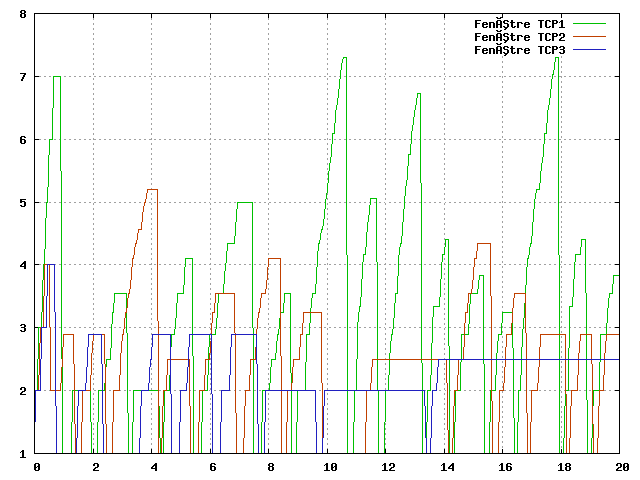
\includegraphics[width=\textwidth]{windowSize}
\end{figure}

\subsection{Longueur de la file d'attente}
\begin{figure}[h]
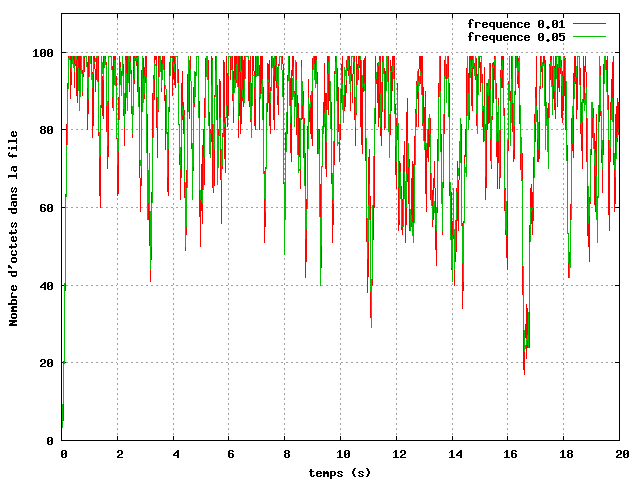
\includegraphics[width=\textwidth]{queueSize}
\caption{Taille de la file d'attente}
\end{figure}

On remarque que la taille de la fenêtre TCP augmente lorsque la file d'attente diminue. La taille de
la fenêtre TCP étant lié aux accusés de réception, le nombre de ces derniers augmente lorsque les
traitement se font plus importants et donc lorsque la taille de la file d'attente diminue.

Un des exemples les plus flagrants a lieu à la $11^e$ seconde, où l'on observe une chute de la
taille de la file d'attente et une fenêtre TCP$_1$ atteignant un pic.

\section{Conclusion}

Ce TP a permis la découverte, plus ou moins laborieuse, du langage Tcl ainsi que la mise en avant du
comportement relativement aléatoire du simulateur ns-2\footnote{On peut par exemple citer le fait
	que la taille des paquets TCP peut être fixée arbitrairement par le simulateur, ou le fait que
certains conflits de paramètres des connexions ne sont pas signalés.}.

De plus, bien que ne sachant pas exactement ce à quoi correspond la taille de la fenêtre TCP, cd TP nous a
permis de mettre en évidence une relation directe entre cette dernière et la taille de la file
d'attente du n\oe uds destinataire.


\vfill
{\raggedleft R\'ealis\'e avec \LaTeX{} \par}



\end{document}
